\subsection{Structural and Physical Analysis}\label{sec:SnP}

\highlight{\begin{table}[ht!]
\centering
\renewcommand{\arraystretch}{2.5}
\begin{tabular}{|c|c|c|}
\hline
\textbf{Source} & \textbf{Basis $g_p(\tau)$} & \textbf{Function} \\
\hline
\multirow{2}{*}{Cable}
    & $\Phi_1(\tau)$ (even)
    & $\displaystyle\sqrt{\frac{2}{\pi}}\,\frac{1}{1+\tau^2}$\\
    & $\Phi_2(\tau)$ (odd)
    & $\displaystyle\sqrt{\frac{2}{\pi}}\,\frac{\tau}{1+\tau^2}$\\
\hline
\multirow{3}{*}{Dipole (Anderson)}
    & $g_{1,1}(\tau)$ (even)
    & $\displaystyle\frac{\sqrt{128/35\pi}}{(1+\tau^2)^{5/2}}$\\
    & $g_{1,2}(\tau)$ (odd)
    & $\displaystyle\frac{\sqrt{128/5\pi}\;\tau}{(1+\tau^2)^{5/2}}$\\
    & $g_{1,3}(\tau)$ (even)
    & $\displaystyle\frac{\sqrt{56/\pi}\;(\tau^2-1/7)}{(1+\tau^2)^{5/2}}$\\
\hline
\multirow{5}{*}{Quadrupole}
    & $g_{2,1}(\tau)$ (even)
    & $\displaystyle\frac{32}{\sqrt{231\pi}\,(1+\tau^2)^{7/2}}$\\
    & $g_{2,2}(\tau)$ (odd)
    & $\displaystyle\frac{-32\,\tau}{\sqrt{21\pi}\,(1+\tau^2)^{7/2}}$\\
    & $g_{2,3}(\tau)$ (even)
    & $\displaystyle\frac{8\sqrt{154}\,(11\tau^2-1)}{77\sqrt{\pi}\,(1+\tau^2)^{7/2}}$\\
    & $g_{2,4}(\tau)$ (odd)
    & $\displaystyle\frac{8\sqrt{6}\,\tau\,(1-3\tau^2)}{3\sqrt{\pi}\,(1+\tau^2)^{7/2}}$\\
    & $g_{2,5}(\tau)$ (even)
    & $\displaystyle\frac{4\sqrt{21}\,(21\tau^4-18\tau^2+1)}{21\sqrt{\pi}\,(1+\tau^2)^{7/2}}$\\
\hline
\end{tabular}
\caption{Comparison of cable, dipole (Anderson), and quadrupole orthonormal basis functions (obtained using the Gegenbauer polynomials formulation from \cite{chenevas2025multipolar}).} 
\label{tab:basis_comparison}
\end{table}
Returning to the statement made in the introduction, MOBFs are designed to represent spatially bounded (compact) sources enclosed within a finite Brillouin sphere. This configuration is fundamentally different from the infinite cable geometry, for which the source effectively extends without bound. In particular, the observation point can never lie outside the Brillouin sphere that encloses the source, and the inability of the MOBF expansion to reproduce the cable’s decay rate is a direct manifestation of this geometric incompatibility.

This discrepancy is readily seen from the analytical expressions in Table~\ref{tab:basis_comparison}. For the cable OBF, the slowest decay rate is of order -1, as exhibited by the function $\phi_2(\tau)$. By contrast, an MOBF of order $M$ belongs to the space
$
\operatorname{span}\!\left\{\frac{\tau^n}{(1+\tau^2)^{M+3/2}}\right\}_{n=0}^{2M},
$
for which the slowest decay rate is given by $2M - 2\left(M+\tfrac{3}{2}\right) = -3$. This decay rate is independent of the multipole order $M$ and is strictly faster than the slowest cable decay rate of $-1$, so no finite multipole order can match the cable's behavior. Consequently, there is no multipole order whose decay matches that of the cable: every multipole decays more rapidly. As a result, any finite truncation of the multipole expansion necessarily fails to capture the full contribution of the field in the far tails.}


\begin{figure}[ht]
\centering

\begin{minipage}{0.75\linewidth}
\centering
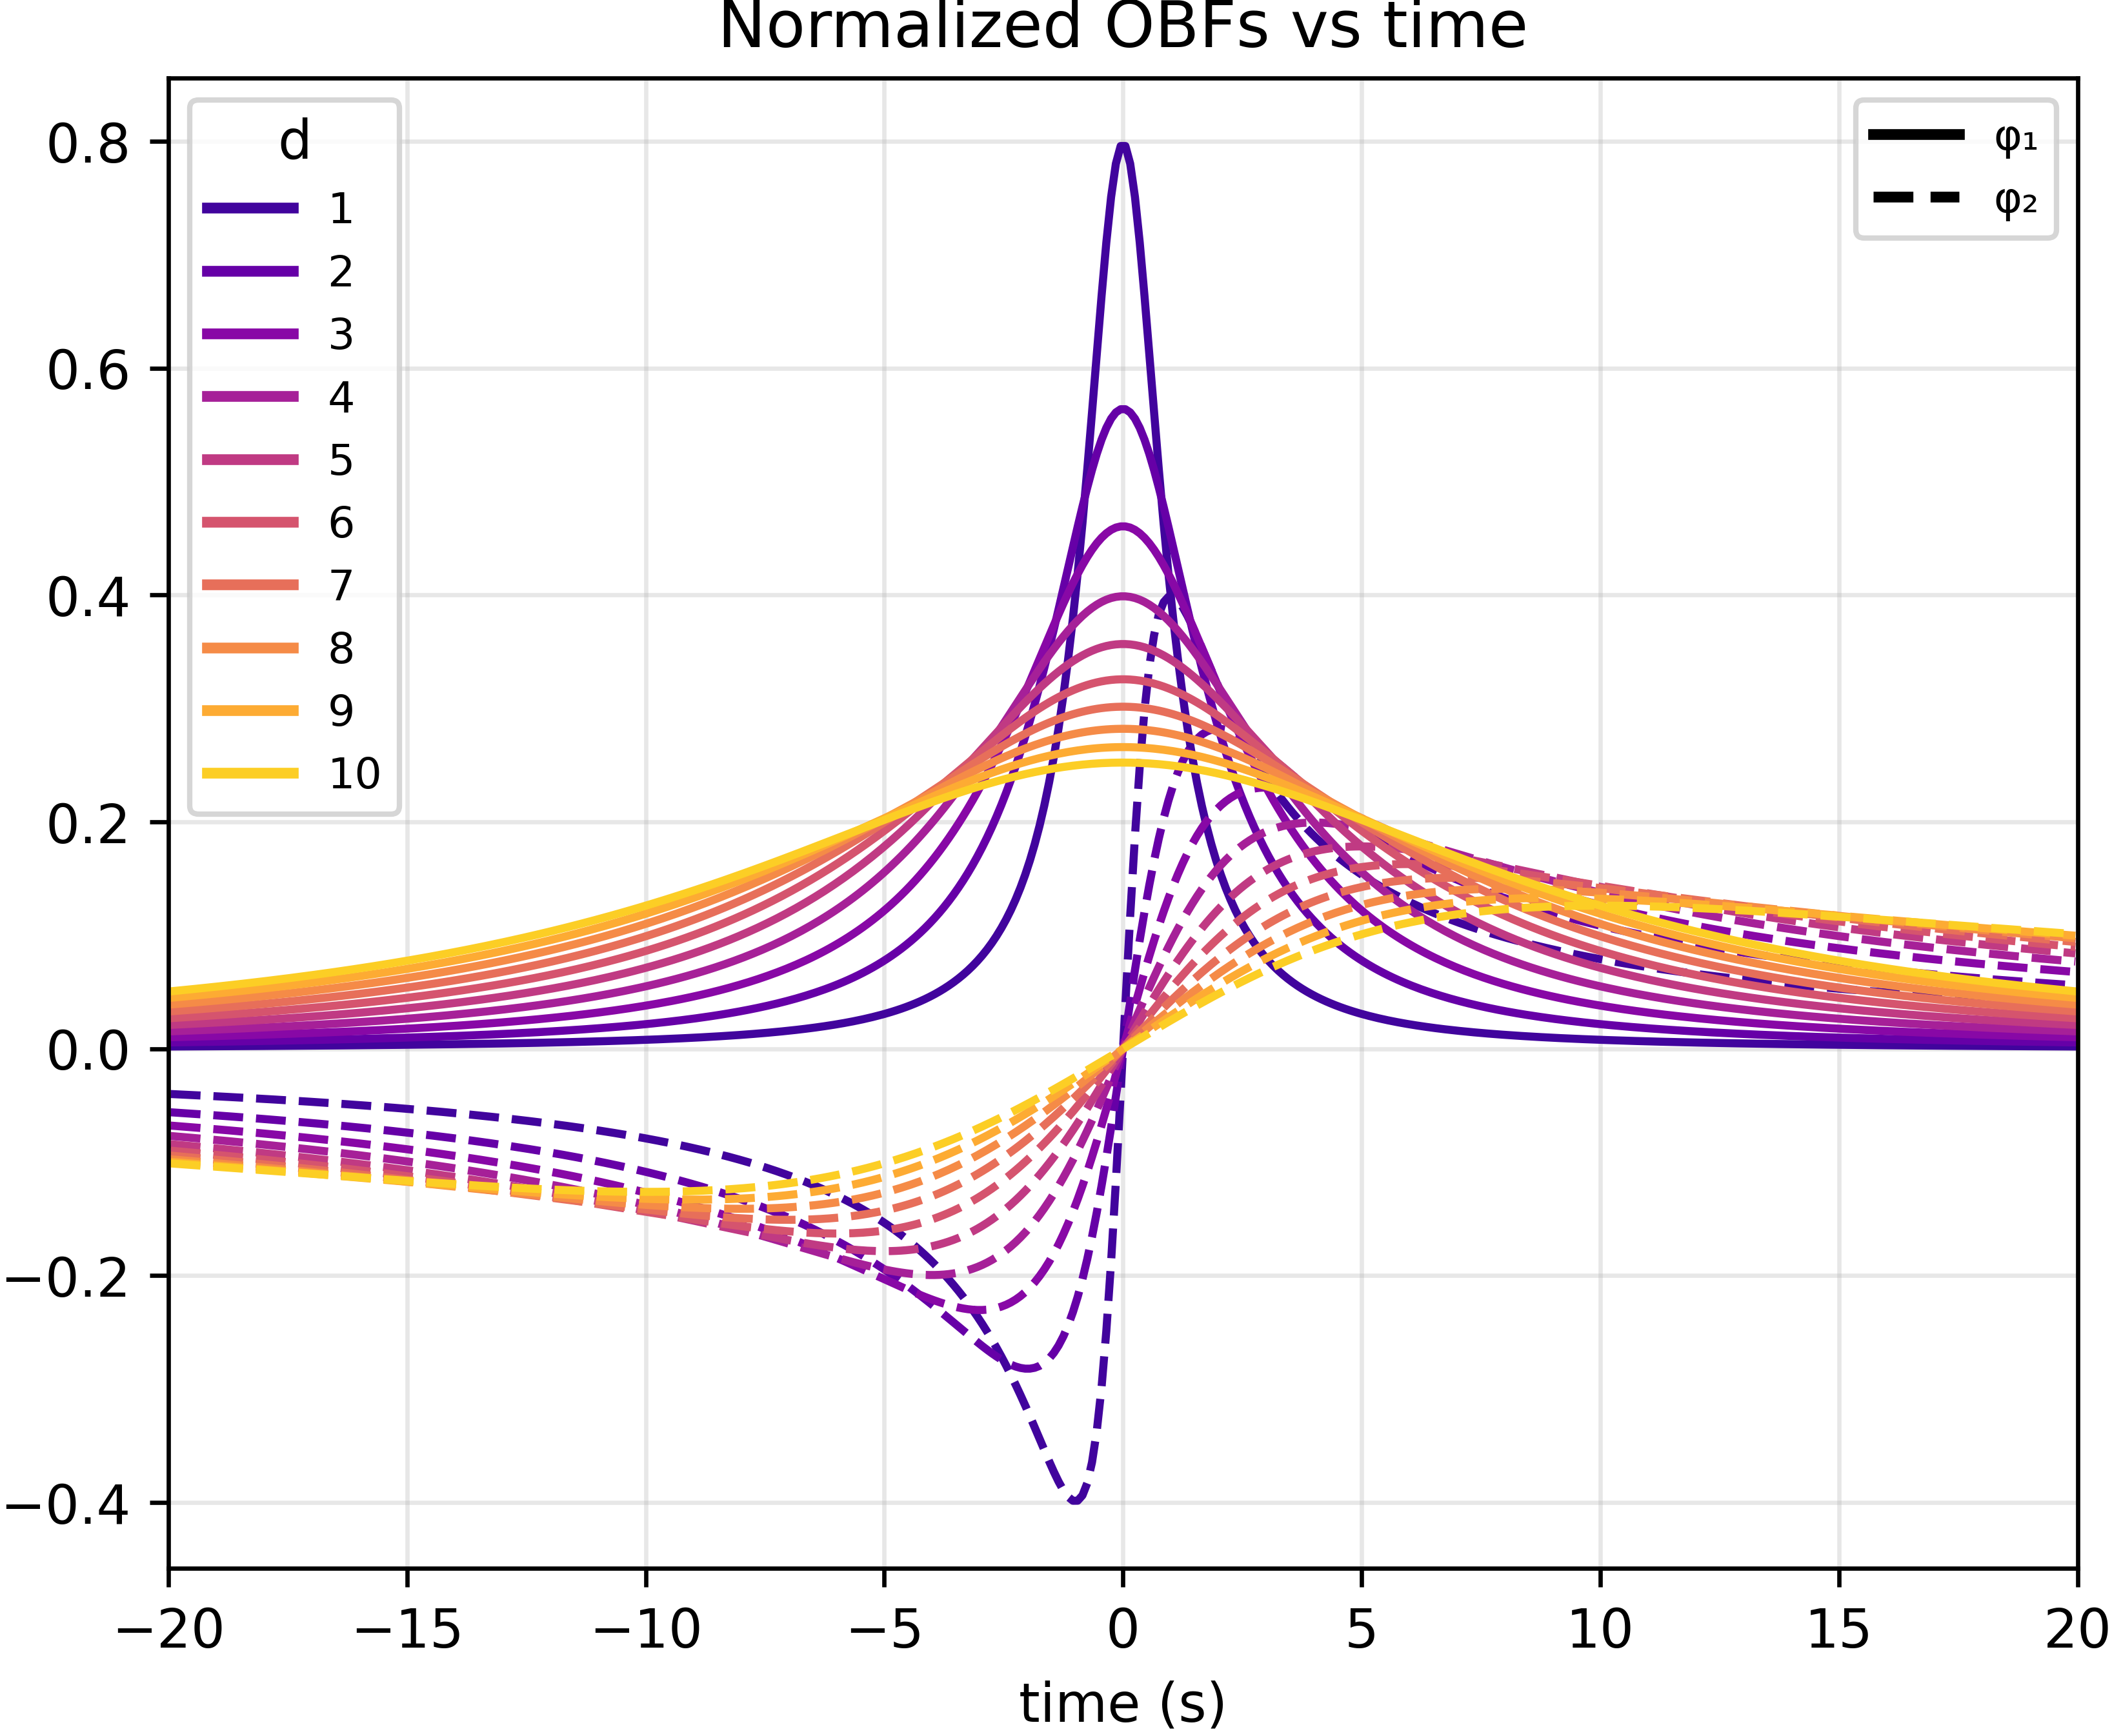
\includegraphics[width=\linewidth]{results_and_discus/figures/OBFs_d_time_normalized.png}
\end{minipage}

\vspace{0.5cm}

\begin{minipage}{0.75\linewidth}
\centering
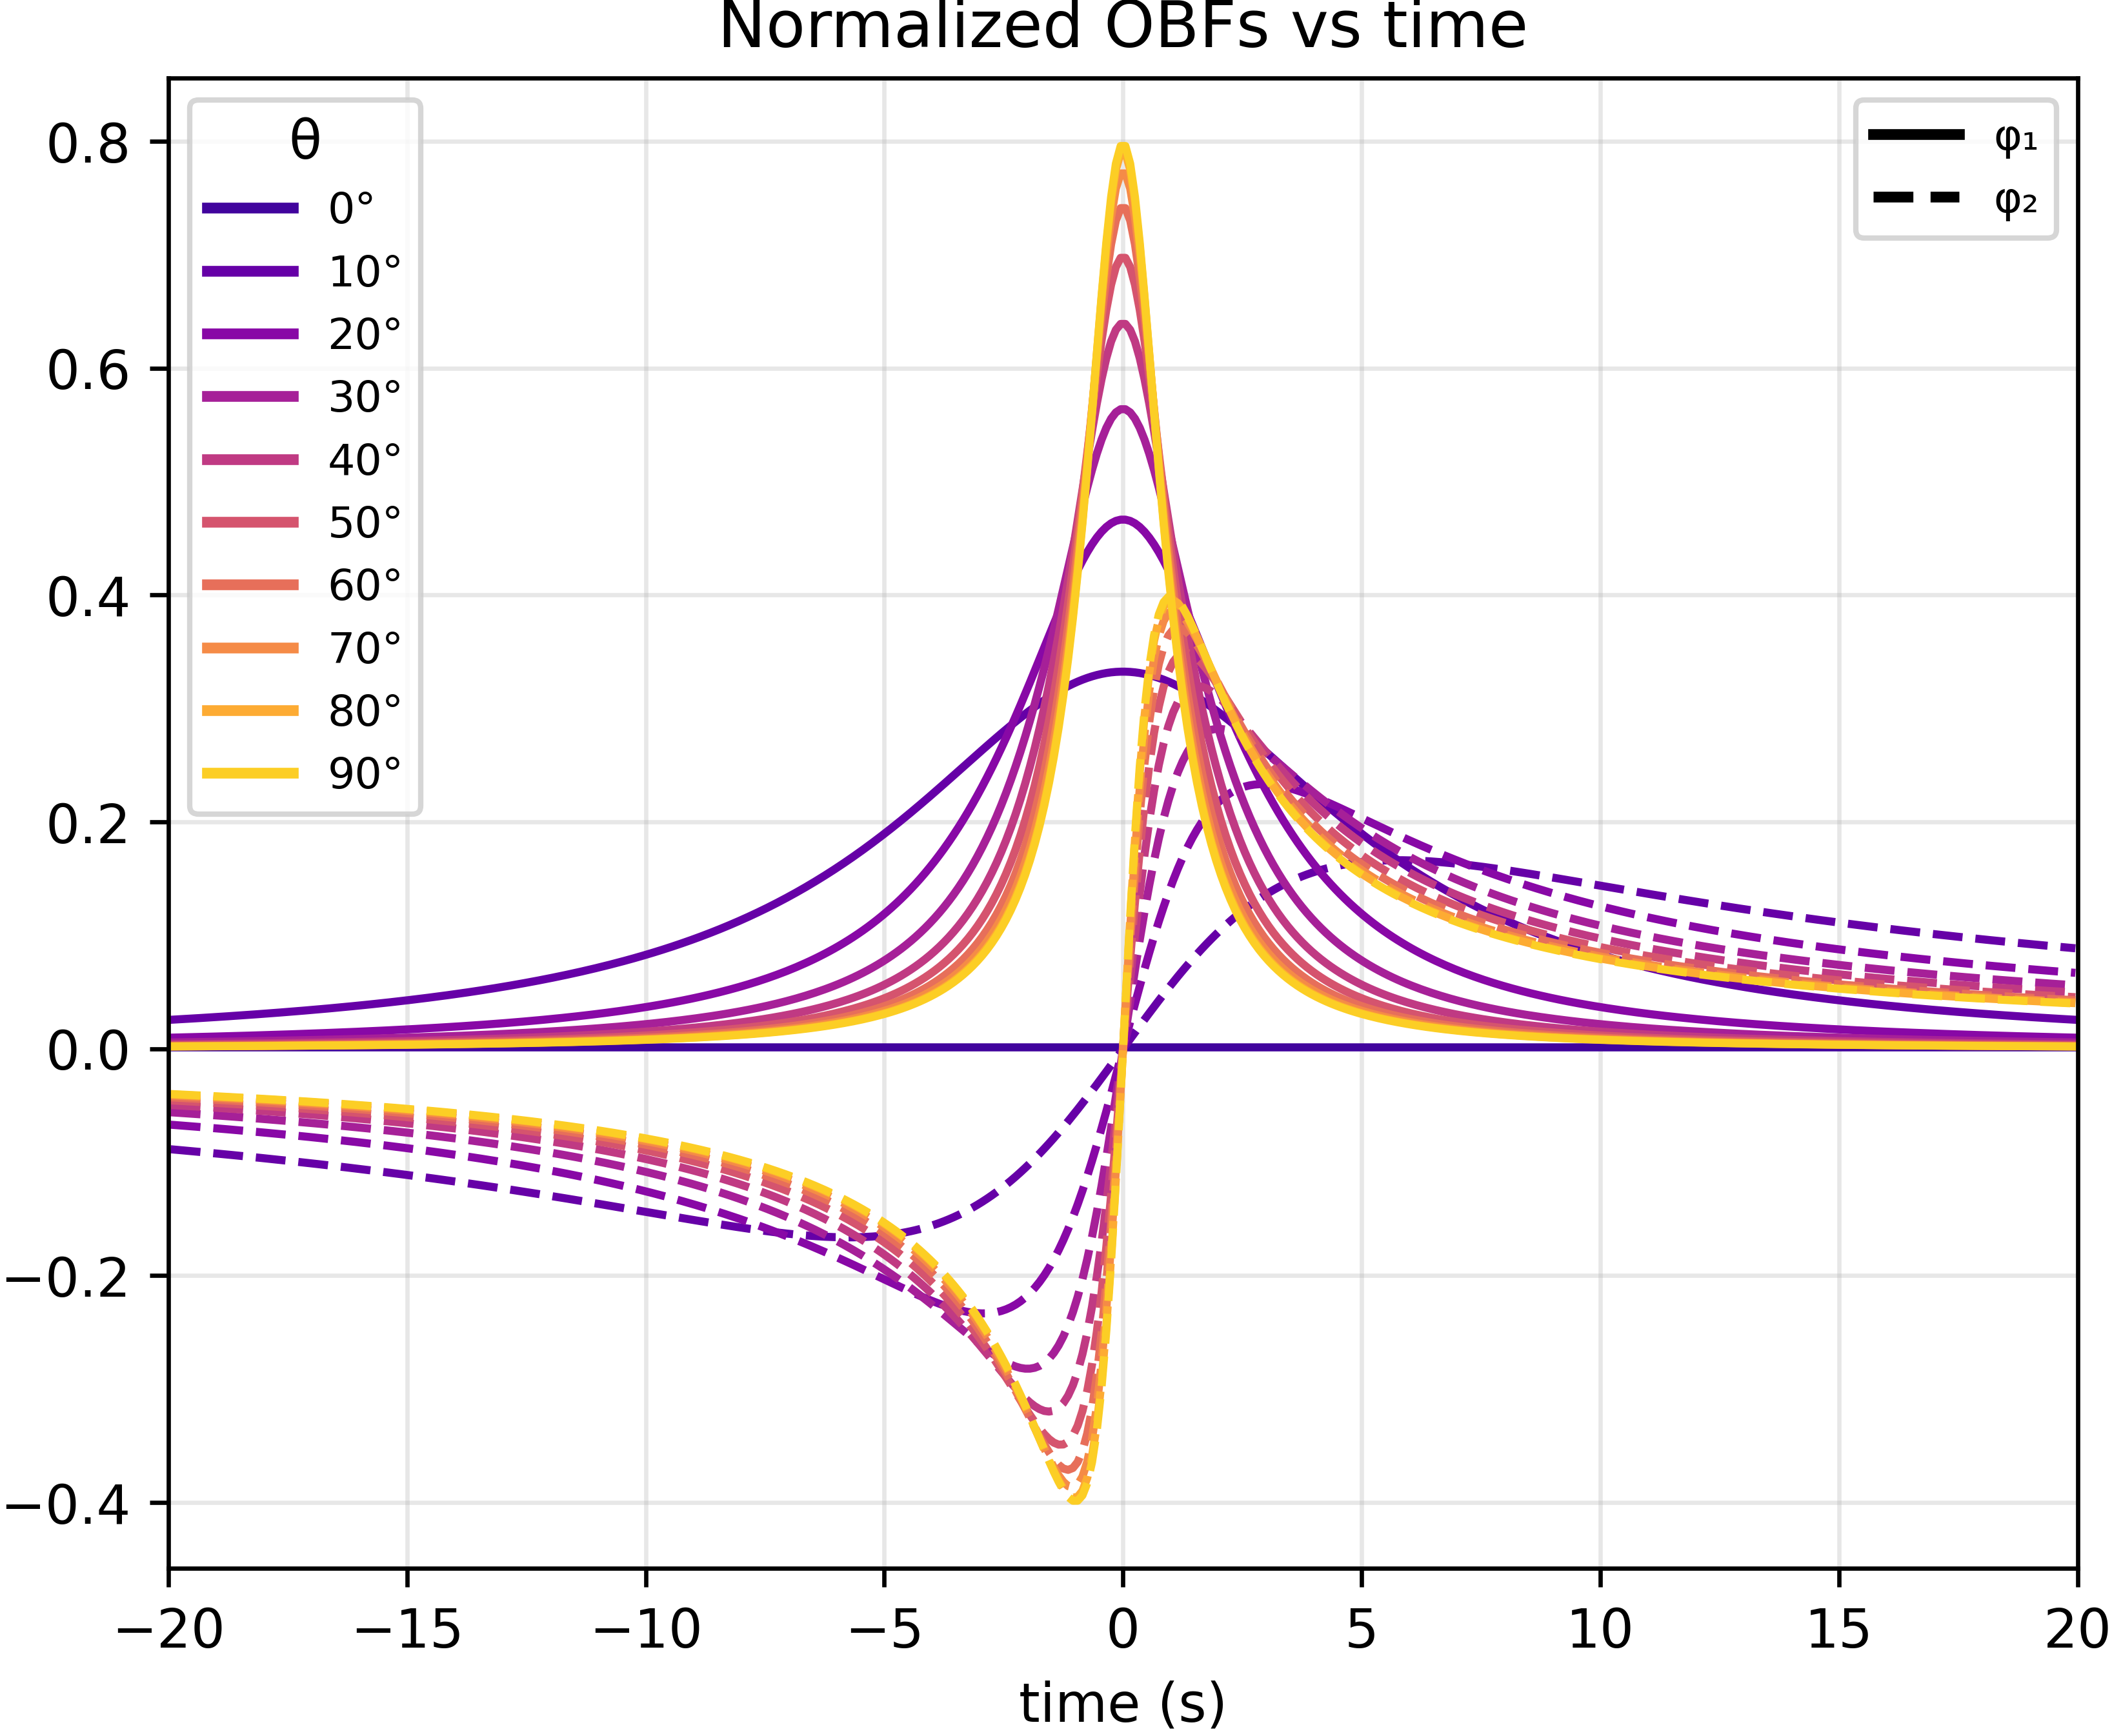
\includegraphics[width=\linewidth]{results_and_discus/figures/OBFs_theta_time_normalized.png}
\end{minipage}

\caption{Time-domain orthonormal basis functions $\Phi_1$ and $\Phi_2$, normalized over energy. Top: Influence of cable depth $d$ (with fixed $\theta = 90^\circ$). Bottom: Influence of trajectory angle $\theta$ (with fixed $d$ = 1).}
\label{fig:OBF_d_theta}
\end{figure}

Regarding cable OBF in isolation, it depends on two unknown parameters $(\frac{v}{d}, \theta)$ where we must assign a prior value for detection, analysis of the basis functions for varying values of $d$ and $\theta$ (see figure \ref{fig:OBF_d_theta}) indicates that their behavior exhibits relatively limited variation in the angular range from \(90^\circ\) to \(40^\circ\), whereas more pronounced changes occur between \(40^\circ\) and \(0^\circ\), a range that is less relevant for detection. This observation suggests a degree of robustness in the choice of the prior value for \(\theta\) before the detection stage. 
Regarding the parameter \(d\), its influence is consistent with that reported in Anderson’s formulation and in \cite{Otnes2007}. Specifically, a relatively large prior uncertainty in \(d\) is acceptable when the source–receiver distance is large. However, as the distance approaches \(\sim 3\,\text{m}\) (which coincides with our operational detection range), the choice of prior becomes increasingly critical, since beyond this threshold the basis functions exhibit pronounced distortion relative to the recorded waveform.

